
\subsection{Data composition and preprocess}
The sequence is represented by the symbol of amino acids such as L, K, M, etc., typically 7-50 in length. Specially, we use 1 to represent the oxidation of methionine (M), and we use 2,3,4 to represent the phosphorylation of serine(S), threonine(T), tyrosine(Y), respectively. In further, we support the peptide with N-terminal acetyl modification. We use the * symbol to indicate modification, @ to indicate no modification. 

For RT datasets, they are comprised of \( \{X, y\} \) pair. 
$X:= \{ <x_0, x_1, x_2, x_3,\dots, x_i, \dots, x_n>\}$. $x_0$ is the symbol of * or @. 
$x_i$ ($i>= 1$) is amino acid. $n$ is the length of peptide. \( y \) is the retention time. 
As the retention time is distributed in the real-world unit, such as minutes or seconds, we scale each dataset by its maximal and minimal of retention time to 0 - 1 by the following formula. 
\[RT_{normalized} = \frac{RT-min(RT)}{max(RT)-min(RT)}\]



Ion intensity datasets are also comprised of \( \{X, y\} \) pair. 
$X := \{ <x_0, x_1, x_2, x_3,\dots, x_i, \dots, x_n, +q> \}$. $+q$
is the charge carried by the peptide sequence before it is fragmented in the mass spectrometer. \( y \) is the spectrum of the peptide. Each y is composed of pairs of key and value.
The key is the ion's name, such as y2+1, b6+2, and the value is their corresponding raw intensity.
We divide each intensity by the maximum of the intensities within a peptide sequence to normalize each intensity into 0-1. As kinds of ions in the dataset is severely imbalanced, we only select the 8 types of ions same as pdeep2, that is b(y)i+1-noloss, b(y)i+2-noloss, b(y)i+1-1,H3PO4 and b(y)i+2-1,H3PO4, i indicating the site of b(y)ion to train and predict. The shape of ion intensity input is illustrated in the supplementary.


%-------------------------------------------------------------------------

 
% %\begin{figure}[t]
%
%   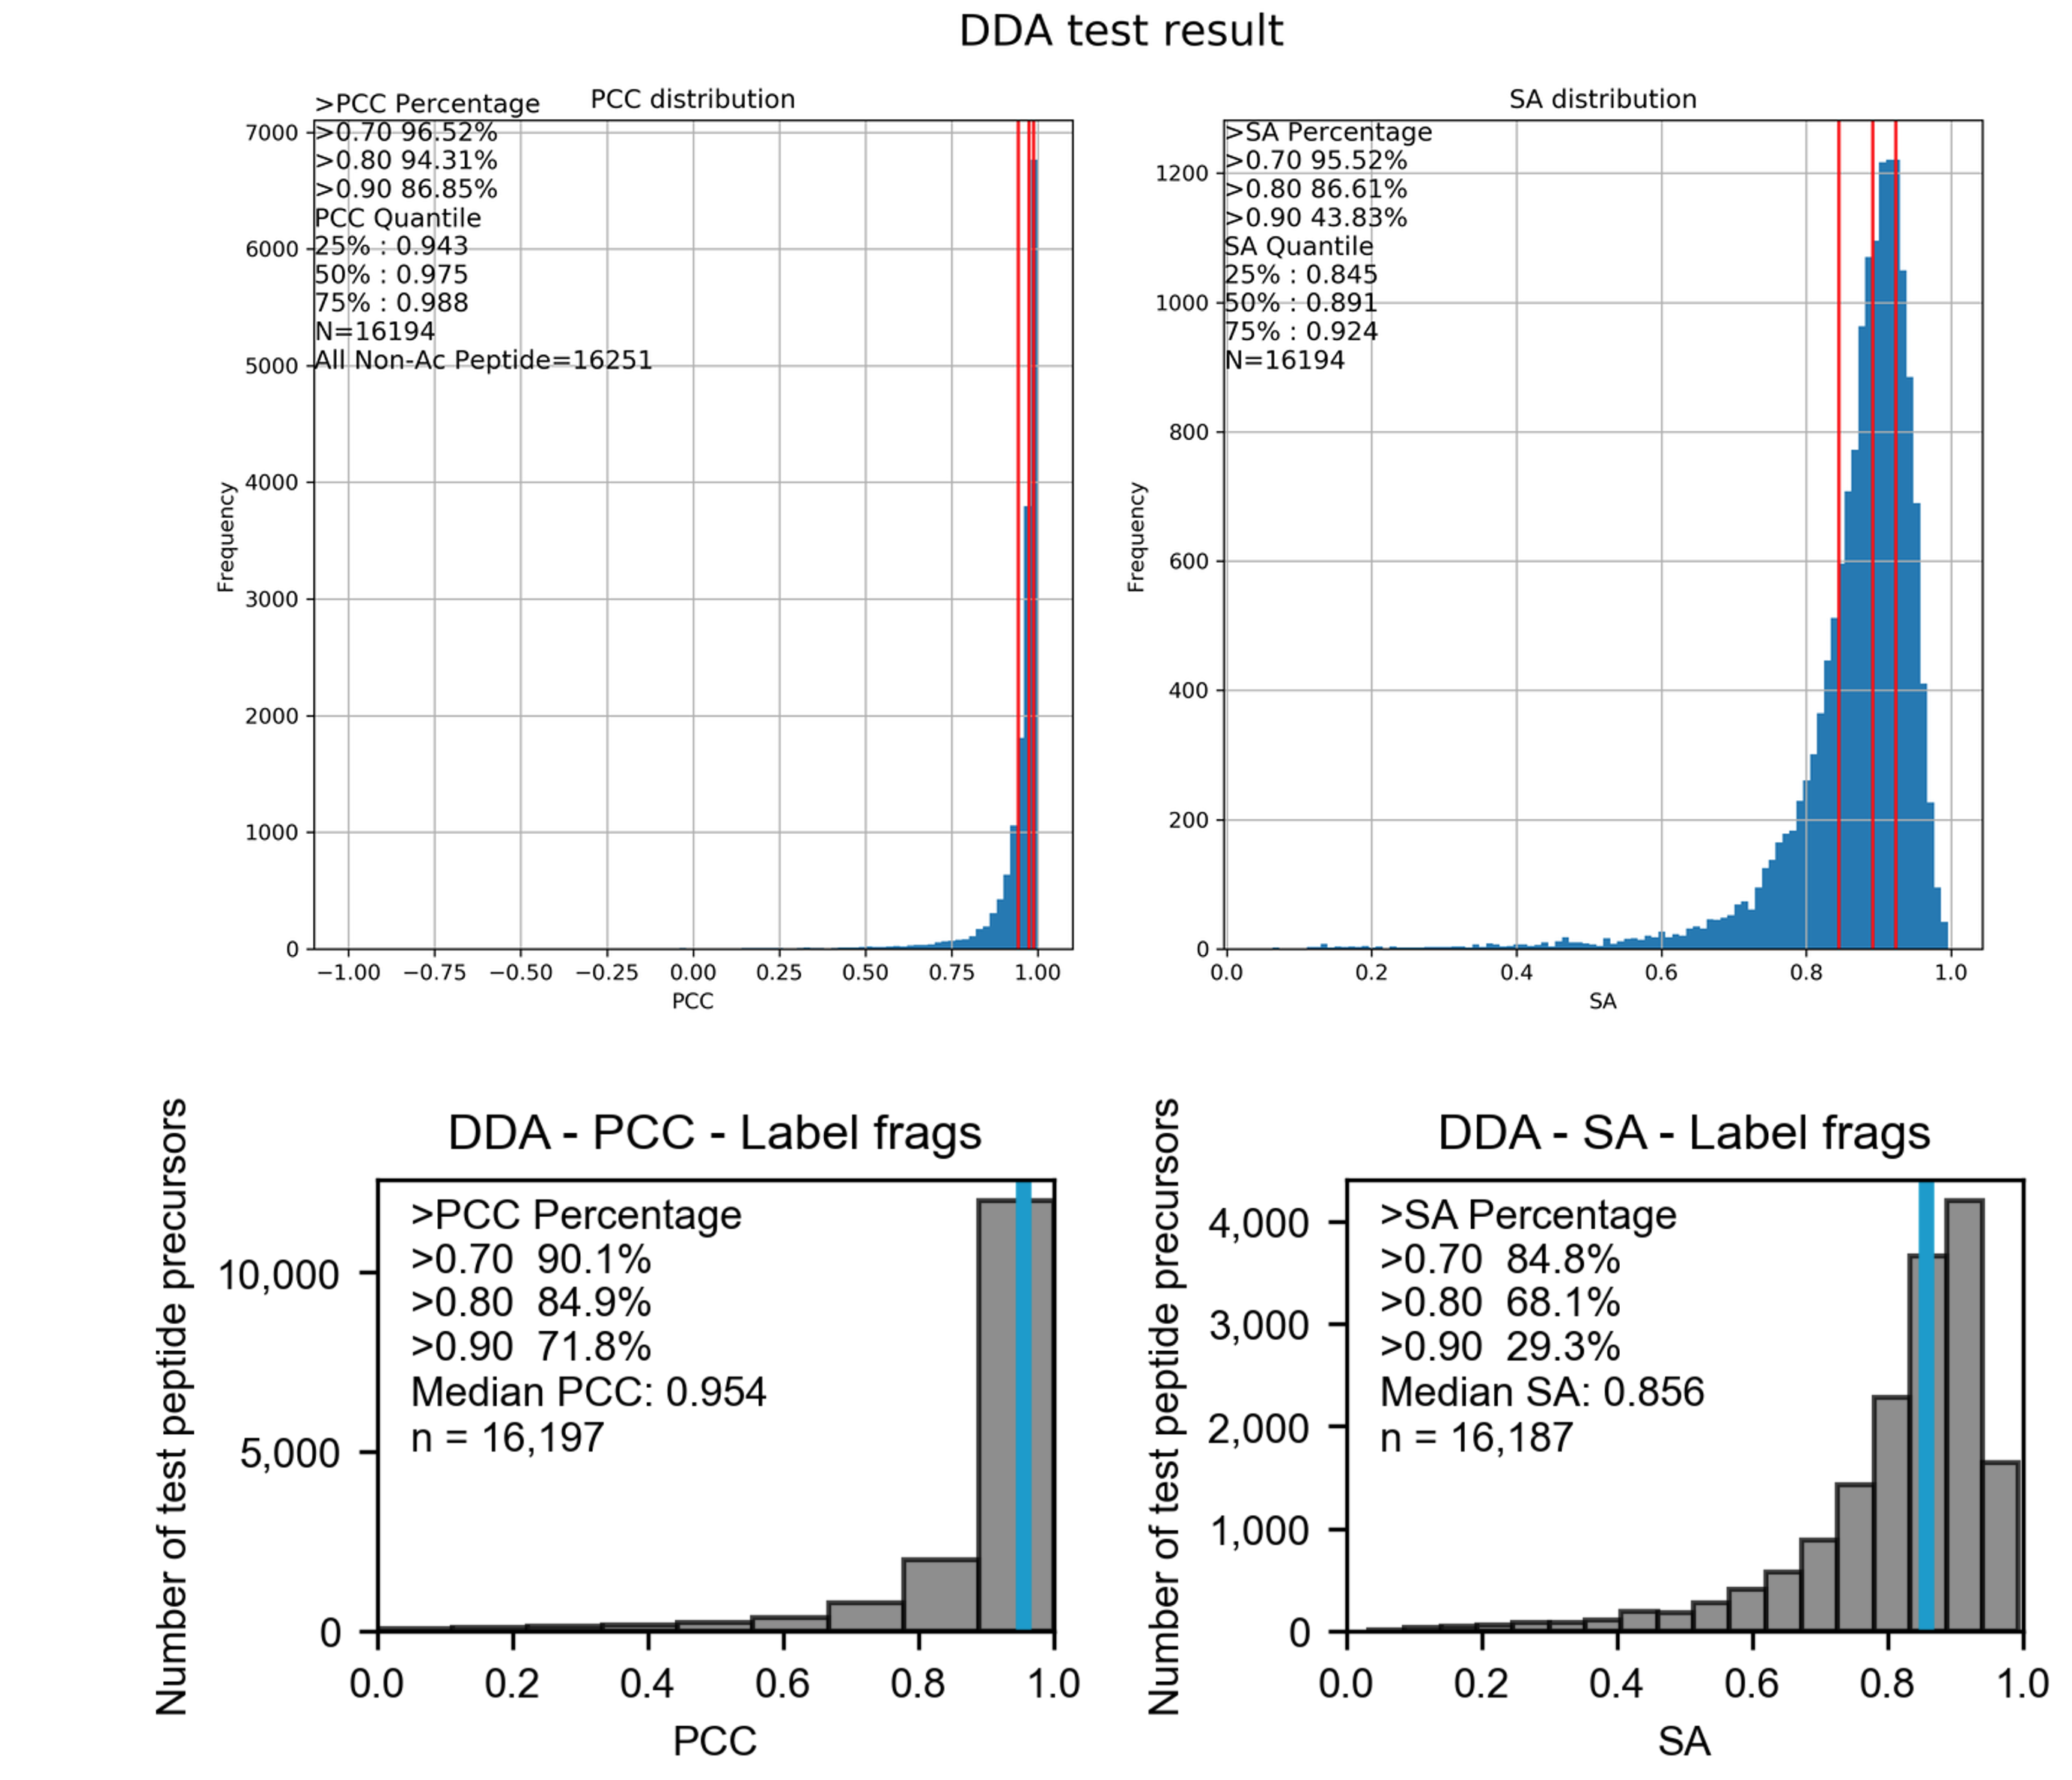
\includegraphics[width=3.0in]{DDA}
%
%   \caption{Visualization of performance of DDA dataset. The above is ours and the below is pdeep2}
%\label{fig:DDA}
%\end{figure}
%
%
%\begin{figure}[t]
%
%   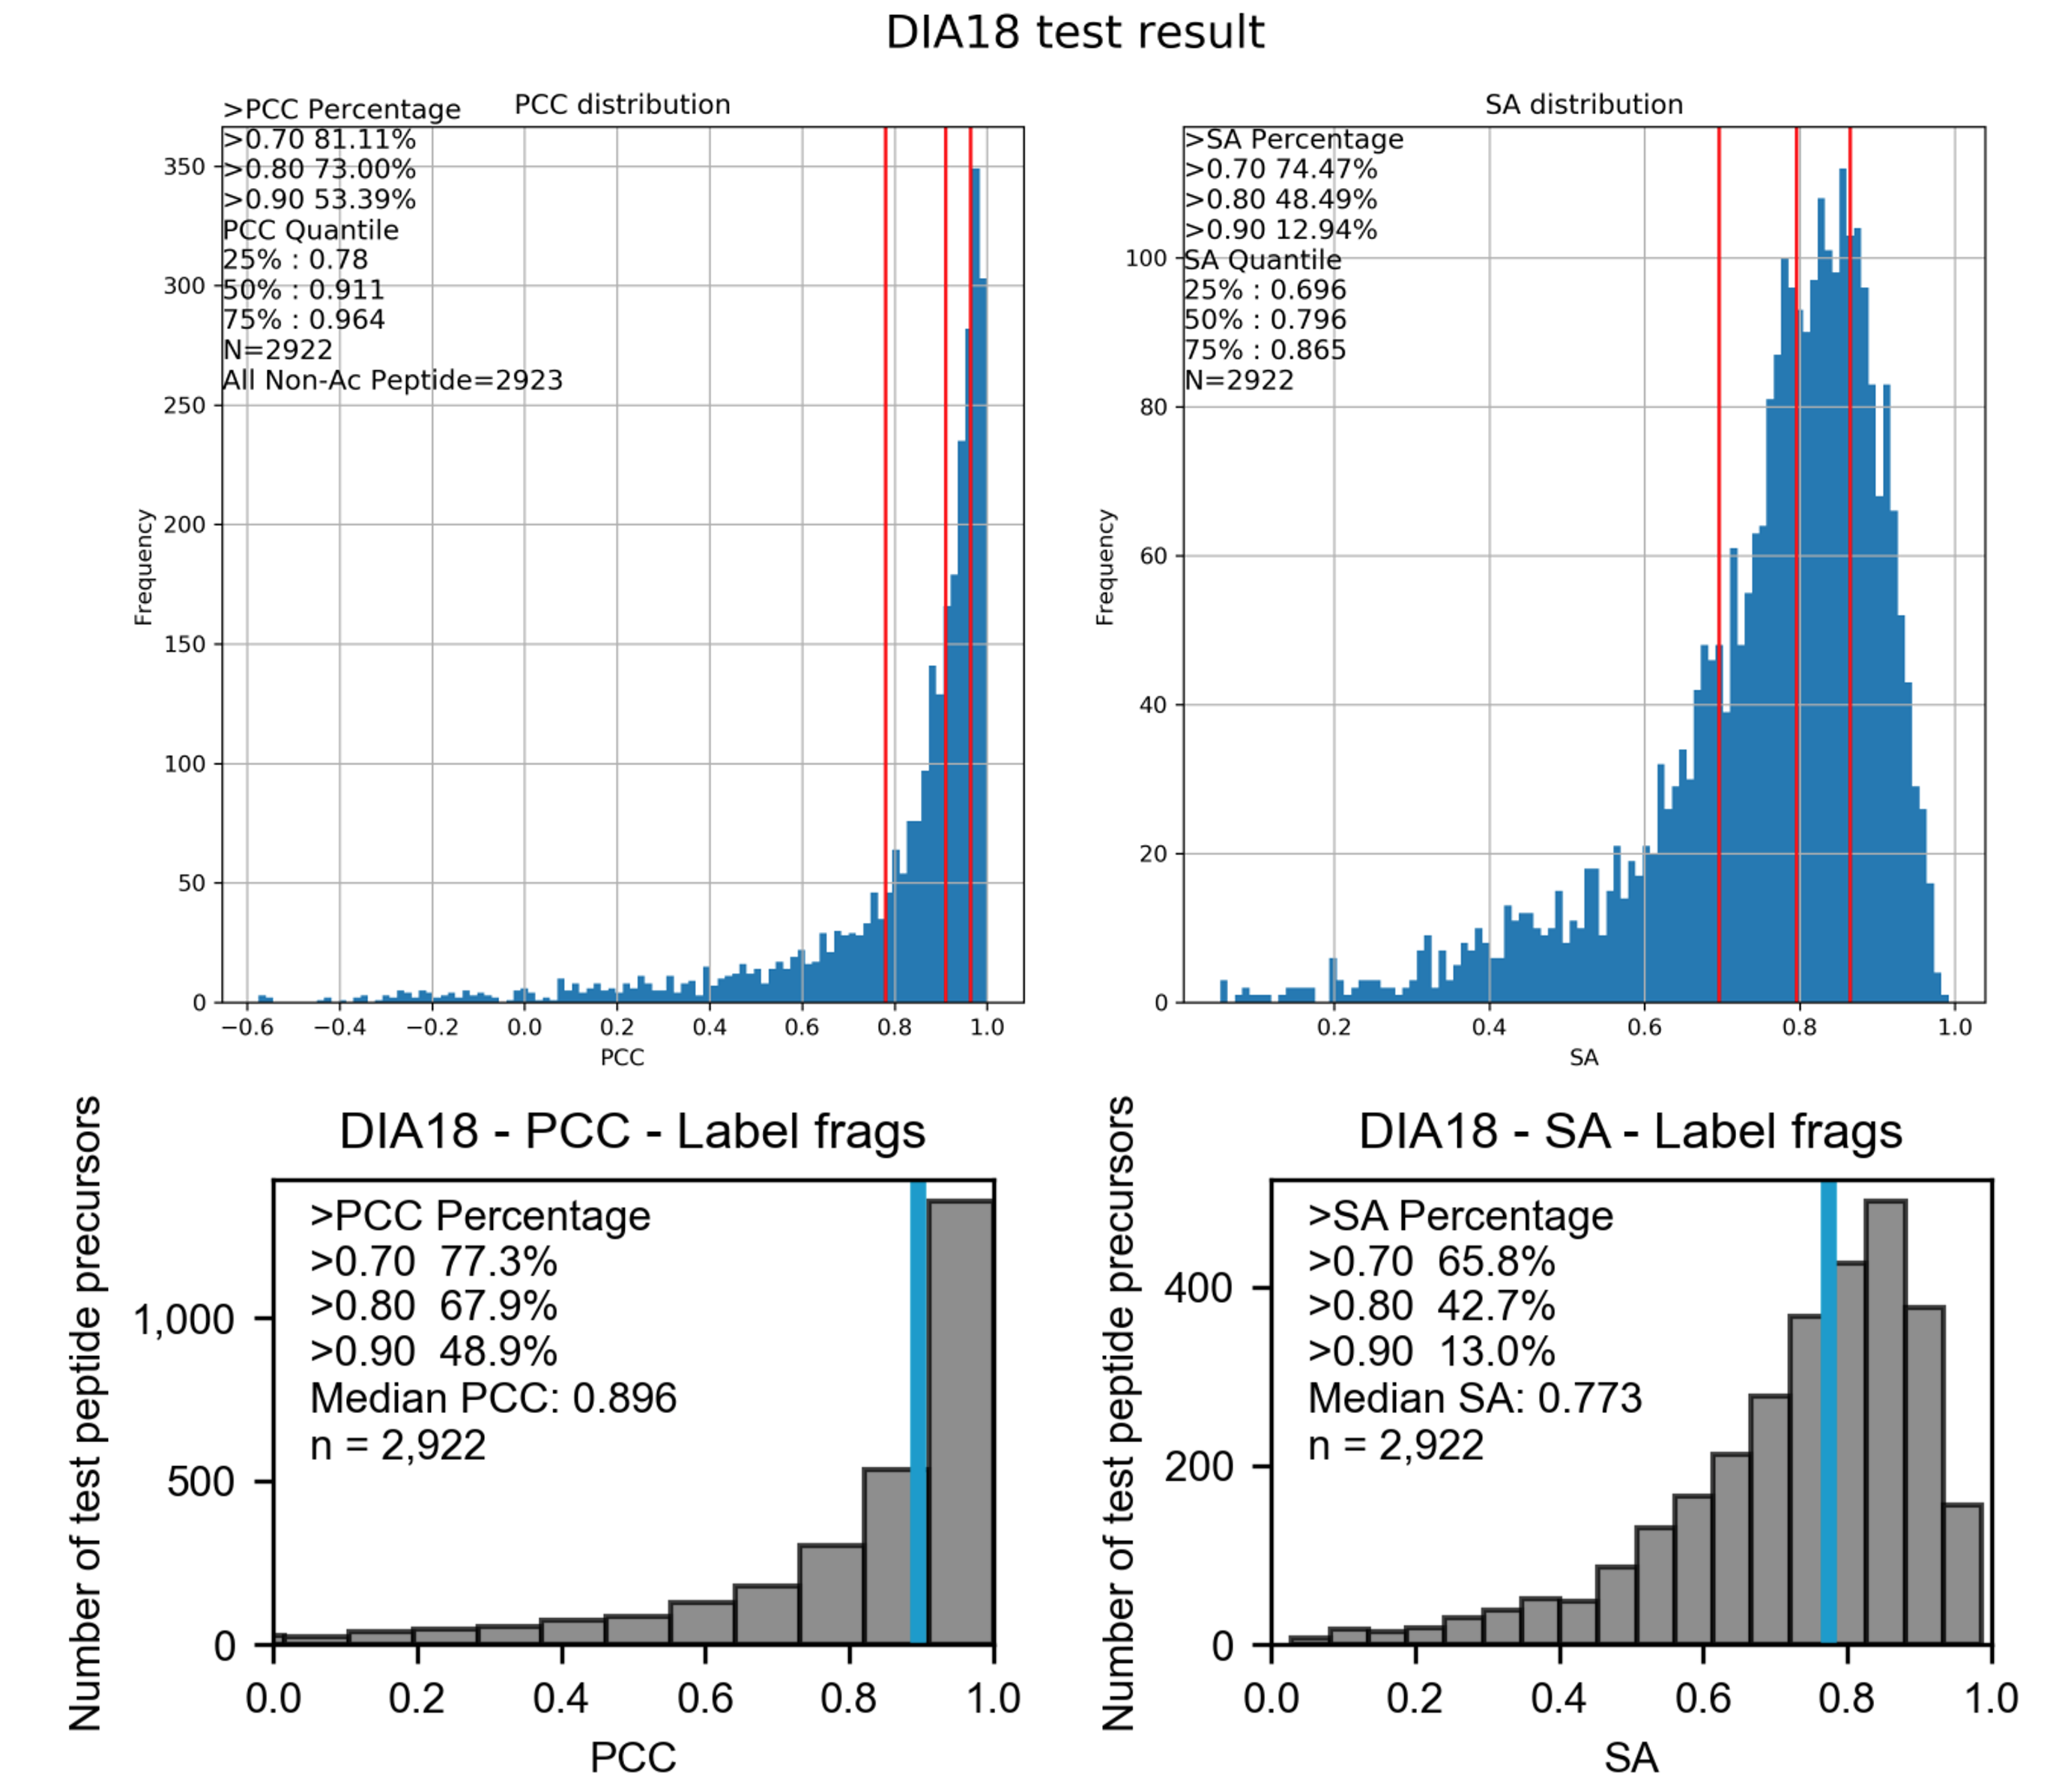
\includegraphics[width=3.0in]{DIA18}
%
%   \caption{Visualization of DIA18 dataset. The above is ours and the below is pdeep2}
%\label{fig:DIA18}
%\end{figure}
%
%
%\begin{figure}[t]
%
%   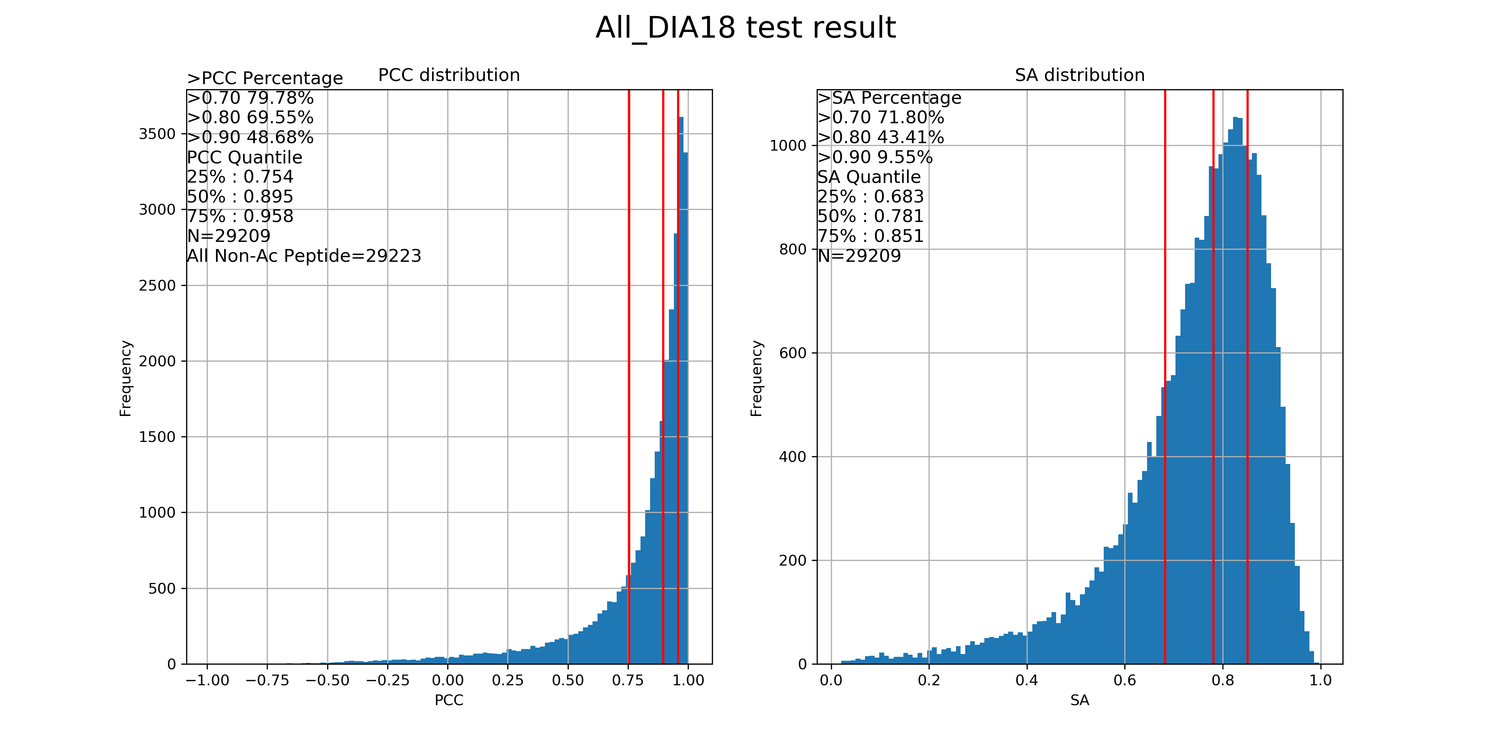
\includegraphics[width=3.5in]{DIA_direct_test}
%
%   \caption{Direct test on DIA18 dataset.}
%\label{fig:DIA18_direct}
%\end{figure}
%

\begin{table}
    \begin{center}
    \begin{tabularx}{\columnwidth}{|m{0.3\columnwidth}|Y|Y|}
    \hline
    data description & no. of peptides & no. of spectra\\
    \hline
    HumanPhosDB~\cite{lawrence2016plug} & 204,558 & -\\
    Jeff~\cite{liu2018vivo} & 67,552 & 89,437\\
    VeroE6~\cite{bouhaddou2020global} & 43,405  & 54,004\\
    R2P2~\cite{leutert2019r2} & 35,808 & 43,312\\
    U2OS-DIA~\cite{wang2020naguider} & 48,327 & 58,843\\
    RPE1-DIA~\cite{bekker2020rapid} & 33,576 & 39,977\\
    RPE1-DDA~\cite{bekker2020rapid} & 129,109 & 165,719\\
    \hline
    \end{tabularx}
    \end{center}
    \caption{Retention time datasets}
    \label{table:Datasets}
    \end{table}
 
    \begin{table}
       \begin{center}
      \resizebox{\columnwidth}{!}$ where the lower is the better, and the right is PCC where the higher is the better.}
       \label{table:Jeff}
       \end{table}
 
 \begin{table}
    \begin{center}
    \begin{tabular}{|l|c|c|}
    \hline
    Model & Median PCC & Median SA \\
    \hline\hline
    pdeep2 & 0.954 & 0.856 \\
    DeepPhospho$\star$ & 0.975 & 0.891 \\
    \hline
    \end{tabular}
    \end{center}
    \caption{DDA Dataset results.Ours is better.}
    \label{table:DDA}
    \end{table}
 
 \begin{table}
    \begin{center}
    \begin{tabular}{|l|c|c|}
    \hline
    Model & Median PCC & Median SA \\
    \hline\hline
    pdeep2 & 0.896 & 0.773 \\
    DeepPhospho$\star$ & 0.911 & 0.796 \\
    \hline
    \end{tabular}
    \end{center}
    \caption{DIA18 Dataset results.Ours is better.}
    \label{table:DIA18}
 \end{table}
 
 \begin{table}
    \begin{center}
    \begin{tabular}{|l|c|c|}
    \hline
    Model & Median PCC & Median SA \\
    \hline\hline
    Direct Test & 0.895 & 0.781 \\
    Train then Test & 0.911 & 0.796 \\
    \hline
    \end{tabular}
    \end{center}
    \caption{DIA18 Dataset results. Direct test only drops little compared to training and test}
    \label{table:DIA18_direct}
 \end{table}
 %%-------------------------------------------------------------------------